% Metódy inžinierskej práce

\documentclass[10pt,twoside,slovak,a4paper]{article}

\usepackage[slovak]{babel}
%\usepackage[T1]{fontenc}
\usepackage[IL2]{fontenc} % lepšia sadzba písmena Ľ než v T1
\usepackage[utf8]{inputenc}
\usepackage{graphicx}
\usepackage{url} % príkaz \url na formátovanie URL
\usepackage{hyperref} % odkazy v texte budú aktívne (pri niektorých triedach dokumentov spôsobuje posun textu)
\usepackage{booktabs}

\usepackage{cite}
%\usepackage{times}

%aby odkazy neboli zvyraznene skaredym 'boxom' ale aby boli iba farebnym pismom-------
\usepackage{xcolor}
%\hypersetup{
%    colorlinks,
%    linkcolor={red!50!black},
%    citecolor={green!70!black},
%    urlcolor={blue!80!black}
%}%------------------------------

%--- popis tabulky nad nou -------------
\usepackage{floatrow}
\floatsetup[table]{capposition=top}
%---------------------------------------

%--- pre dvojitý bullet-point zoznam---
\usepackage{multienum}
\newenvironment{multiitem}{%
  \multienumerate\renewcommand{\labelname}{\textbullet}%
}{%
  \endmultienumerate%
}
%--------------------------------------

\pagestyle{myheadings}

\title{Nástroje CASE a ich využitie v reverznom inžinierstve\thanks{Semestrálny projekt v predmete Metódy inžinierskej práce, ak. rok 2021/22 vedenie: Vladimír Mlynarovič}} % meno a priezvisko vyučujúceho na cvičeniach

\author{Šimon Ukuš\\[2pt]
	{\small Slovenská technická univerzita v Bratislave}\\
	{\small Fakulta informatiky a informačných technológií}\\
	{\small \texttt{xukus@stuba.sk}}
	}

\date{\small 9. december 2021} 



\begin{document}

\maketitle

\begin{abstract}
Článok sa zaoberá problematikou softvérového inžinierstva, kontkrétne ako je možné proces vývoja softvéru automatizovať pomocou nástrojov CASE - Computer-Aided Software Engineering (Počítačom podporované softvérové inžinierstvo). V práci sa uvádza klasifikácia týchto nástrojov.  Článok ďalej skúma softvérové inžinierstvo a použitie CASE nástrojov z inej perspektívy.  Na rozdiel od vnímania vývoja softvéru klasicky, teda smerom vpred (Forward Engineering) sa sústredí na tzv. spätné inžinierstvo (Reverse Engineering). Tu je skúmaná kompletnosť a presnosť spätne navrhnutých UML diagramov generovaných nástrojmi CASE. Predmetom porovnania bolo celkom 8 nástrojov (z toho 6 open source a 2 komerčné). Tieto nástroje boli hodnotené na základe toho, aké typy vstupov podporujú, aké typy diagramov dokážu rekonštruovať a v akej kvalite.
 \\
 \\
 Kľúčové slová: nástroje CASE, softvérové inžinierstvo, reverzné inžinierstvo, UML model, modelovanie v softvérovom inžinierstve
 \\
 \\
\end{abstract}


\section{Úvod}
Pojem softvérové inžinierstvo môže byť chápaný ako uplatňovanie metód, postupov a nástrojov na riadenie a vývoj počítačových systémov~\cite{1985}. Ide o komplexný postup, na ktorom sa zúčastňuje mnoho odborníkov z rôznych oblastí, ako napríklad projektový manažér, team líder, softvérový developer, tester, UI dizajnér a mnoho ďalších. Časť ich práce je možno automatizovať či uľahčiť využitím nástrojov CASE. Tieto nástroje sú špeciálne vyvinuté pre podporu vývoja softvéru, automatizujú proces vývoja. Cieľom ich implementácie je ušetrenie času a nákladov pri vývoji softvéru a zvýšenie jeho kvality~\cite{Osama:Adoption}.

Využitie nástrojov CASE a ich klasifikácia sú uvedené v časti~\ref{klasifikácia}., kde je popísané delenie podľa toho, ktorú časť tzv. životného cyklu vývoja softvéru (Software Development Life Cycle, ďalej len SDLC) pomájhajú automatizovať. 
V časti~\ref{forward vs reverse} sa čitateľ zoznámi s pojmom \emph{reverzné inžinierstvo}. Nachádza sa tu prehľad, v ktorom je popísaný rozdiel medzi tzv. \emph{forward} (dopredným) a \emph{reverse} (spätným) inžinierstvom. 
Samotné nástroje, ich predstavenie a následné porovnanie rozoberajú časti~\ref{predstavenie}~a~\ref{porovnanie}.
Záverečné hodnotenie týchto nástrojov prináša časť~\ref{zhrnutie}.



\section{Klasifikácia nástrojov CASE}\label{klasifikácia}

% tento odstavec by bolo možné nahradiť reakciou na tému ``Technológia a ľudia''
Nástroje CASE sú odpoveďou na stále narastujúce nároky a zvyšujúcu sa komplexnosť počítačových systémov. Podporujú vývoj softvéru a dajú sa aplikovať v niektorých, niekedy vo všetkých fázach SDLC, ktorého podpora je čoraz žiadúcejšia. Náklady na vývoj softvéru každým rokom narastajú, a preto čo i len skromné vylepšenia pri vývoji a automatizácii môžu znamenať veľké úspory.  Sú cielené na riešenie ťažkostí pri vývoji vysokokvalitného a komplexného softvéru načas a v súlade s rozpočtom~\cite{2001}. \\

Ako sa vyššie spomína, nástroje CASE slúžia na podporu rôznych fáz SDLC, prípadne dokážu automatizovať všetky z nich. Zvyknú sa preto klasifikovať podľa toho, ktoré štádium životného cyklu podporujú. Takéto rozdelenie vyzerá nasledovne:

\begin{itemize}
\item Upper CASE nástroje
\item Lower CASE nástroje
\item Integrated CASE nástroje
\end{itemize}
\textbf{Upper CASE}, niekedy označované aj ako \emph{front end CASE} slúžia na podporu skorých fáz životného cyklu softvéru, napríklad pri analýze a dizajne.\\
\textbf{Lower CASE}, tiež nazývané aj \emph{back end CASE} zase nachádzajú využitie v neskorších fázach životného cyklu softvéru, najmä pri testovaní a vytváraní kódu.\\
\textbf{Integrated CASE}, sú schopné pokryť obe časti SDLC~\cite{1998}.


Iný pohľad na kategorizáciu poskytuje autor~\cite{2017}, ktroý nespája fázy SDLC do tzv. skorých a neskorších, ale konkrétne fázy jednotlivo vymenúva a podľa toho delí nástroje CASE ako nástroje na:
\begin{multiitem}
\mitemxx {riadenie projektov}{nástroje formálnych metód}
\mitemxx {analýzu a návrh}{Klient/Server nástroje}
\mitemxx {podporu Objektovo- Orientovaného sw inžinierstva}{webové inžinierstvo}
\mitemxx {testovanie}{opätovné inžinierstvo (Reengineering)}
\end{multiitem}

Pri tomto delení sa stretávame s pojmom opätovné inžinierstvo (Reengineering), a keďže v ďalších kapitolách je rozpracovaná téma reverzného inžinierstva a použitie nástrojov CASE v reverznom (spätnom) inžinierstve, je potrebné uviesť, že je rozdiel medzi spätným inžinierstvom (Reverse Engineering) a opätovným inžinierstvom (Reengineering). Síce oba pojmy odkazujú na ďalšie skúmanie alebo vývoj už hotových produktov, metódy a požadované výsledky sa výrazne líšia.  Ako~\cite{reengineering} ďalej vysvetľuje, reverzné inžinierstvo sa snaží odhaliť, ako daný systém funguje. Úlohou opätovného inžinierstva je zlepšenie súčasného návrhu skúmaním jeho konkrétnych aspektov. 


\section{Z dopredného inžinierstva k spätnému}\label{forward vs reverse}


Spätné inžinerstvo, ako už bolo v sekcii~\ref{klasifikácia} spomenuté, sa snaží pochopiť funkciu systému. Obr. \ref{obr_forward_reverse} ilustruje spôsob vývoja informačných systémov. Pre jednoduchosť boli použité tri fázy životného cyklu, kde prvá -  \emph{"požiadavky"} predstavuje špecifikáciu problému, druhá  - \emph{"dizajn"} zase špecifikáciu riešenia a tretia -  \emph{''implementácia"} predstavuje programovanie a testovanie požadovaného systému.


Pojem dopredné \textit{(forward)} inžinierstvo reprezentuje tradičný proces vývoja softvéru, kedy sa postupuje od prvotných abstraktných modelov, cez dizajn až ku konečnej implementácii systému. Zavedenie názvu pre niečo tak priamočiare sa môže zdať zbytočné, možno aj mätúce . V našom prípade, a tiež v mnoho iných, je to však nevyhnutné pre jeho odlíšenie od spätného inžinierstva. Ako Obr \ref{obr_forward_reverse} ukazuje, dopredné inžinierstvo prechádza jednotlivými fázami SDLC z ľava do prava.
\begin{figure}[h]
\centering
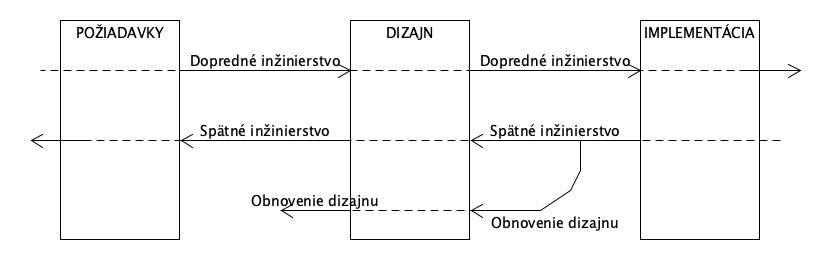
\includegraphics[width=0.85\textwidth]{forward_reverse.jpg}
\caption{Vybrané fázy SDLC a znázornené procesy súvisiace s dopredným a spätným inžinierstvom (prevzaté a preložené z~\cite{2010})}
\label{obr_forward_reverse}
\end{figure}

Na druhej strane, spätné \textit{(reverse)} inžinierstvo postupuje opačným smerom oproti doprednému inžinierstvu, čo ilustruje Obr.  \ref{obr_forward_reverse}. 
Reverzné inžinierstvo je proces, počas ktorého je systém (softvér) analyzovaný, výsledkom čoho je pochopenie fungovania daného systému, identifikácia komponentov, prípadne prinavrátenie stratených informácií \cite{2010}.
Vďaka reverznému inžinierstvu je možné rekonštruovať UML diagramy, na čo je možné použiť nástroje CASE. Práve problematika generovania UML diagramov zo zdrojového kódu je ďalej popísaná v sekciách \ref{predstavenie} a \ref{porovnanie}, pre ktoré bola podkladom štúdia
realizovaná Osmanom et al. \cite{Osman:RE}. 

%-- Tu by sa prípadne hodil odstavec s reakciou na tému ``Udržateľnosť a etika''

\section{Predstavenie nástrojov}\label{predstavenie}

Táto sekcia zobrazuje nástroje, ktoré boli predmetom skúmania, realizovaného autorom~\cite{Osman:RE}. Všetkých 8 posudzovaných nástrojov je uvedených v Tabuľke~\ref{tabulka1}. Pri evaluácii komerčných nástrojov bola použitá verzia pre účely testovania, prípadne verzia na vzedlávacie účely.

%tabulka:
\begin{table}[h]
\centering
\makebox[\textwidth][c]{
\begin{tabular}{|c|c|c|c|c|}
\hline
\textbf{č} & \textbf{nástroj CASE} & \textbf{informácie} & \textbf{Predajca} & \textbf{Typ Licencie}\\
\hline
1 & Visual Paradigm 8.1 & \href{http://www.visual-paradigm.com/}{Visual Paradigm} & Visual Paradigm & Komerčné\\
\hline
2 & MagicDraw 17.0 & \href{http://www.magicdraw.com/}{MagicDraw} & No Magic & Komerčné\\
\hline
3 & Altova Umodel 2011 & \href{http://www.altova.com/}{Altova Umodel} & Altova& Komerčné\\
\hline
4 & Enterprise Architect 8.0 & \href{http://www.sparxsystems.com.au/}{Enterprise Architect} & Sprax System & Komerčné\\
\hline
5 & Rational Software Architect 8.0.1 & \href{https://www.ibm.com/products/rational-software-architect-designer}{Rational Software} & IBM & Komerčné\\ 
\hline
6 & MyEclipse 8.6 & \href{https://www.genuitec.com/products/myeclipse/features/}{MyEclipse} & Genuitec & Komerčné\\
\hline
7 & StarUML 5 & \href{http://staruml.sourceforge.net/}{StarUML} &StarUML & Open Source\\
\hline
8 & ArgoUML & \href{https://argouml-tigris-org.github.io/tigris/argouml/tours/}{ArgoUML} & Tigris.org & Open Source\\
\hline
\end{tabular}
}
\caption{Zoznam posudzovaných nástrojov (prevzaté a preložené z~\cite{Osman:RE})}\label{tabulka1}
\end{table}

Pri porovnávaní nástrojov boli zisťované nasledovné parametre:
\begin{itemize}
\item ktoré programovacie jazyky sú podporované jednotlivými nástrojmi
\item ktoré nástroje sú schopné rekonštrukcie ktorých diagramov (diagramy balíčkov - 'package'; diagramy tried - 'class'; sekvenčné diagramy - 'sequence')
\item či sú rekonštruované diagramy správne a úplne
\end{itemize}

%\pagebreak
\section{Výsledky porovnania nástrojov}\label{porovnanie}

V tejto sekcii sú uvedené výsledky porovnania nástrojov zo sekcie \ref{predstavenie}. Výsledky sú zhrnuté v Tabuľke \ref{tabulka2}.

Nástrojmi podporované programovacie jazyky sú uvedené v Tabuľke \ref{tabulka2}, z ktorej je možné vyčítať, že Enterprise Architect podporuje všetky jazyky uvedené v hlavičke tabuľky. Celkovo väčšina nástrojov dokáže rekonštruovať UML modely zo súborov zdrojových kódov typu .java, .cpp, .cs. Dokonca všetky porovnávané nástroje dokážu spätne generovať modely zo zdrojových kódov napísaných v jazyku Java.

V pravej časti Tabuľky \ref{tabulka2} sú uvedené schopnosti nástrojov z hľadiska podporovaných typov diagramov. V tejto časti tabuľky sa vyskytujú tri rôzne znaky, ktoré predstavujú tri úrovne hodnotiacej škály. Vysvetlivky k danej škále sú nasledovné \cite{Osman:RE}:
\begin{itemize}
\item ``+'' - nástroj dokáže rekonštruovať daný typ diagramu aj keď s malou/malými chybami, ako napríklad nesprávne uvedenie/neuvedenie vzťahov pri diagramoch tried (agregácia a kopozícia často uvedená ako asociácia)

\item ``0'' - nástroj síce dokáže rekonštruovať daný typ diagramu, ale neposkytuje všetky informácia o diagrame

\item ``-'' - nástroj nie je schopný rekonštrukcie daného typu diagramu

\end{itemize}

\begin{table}[h]
\centering
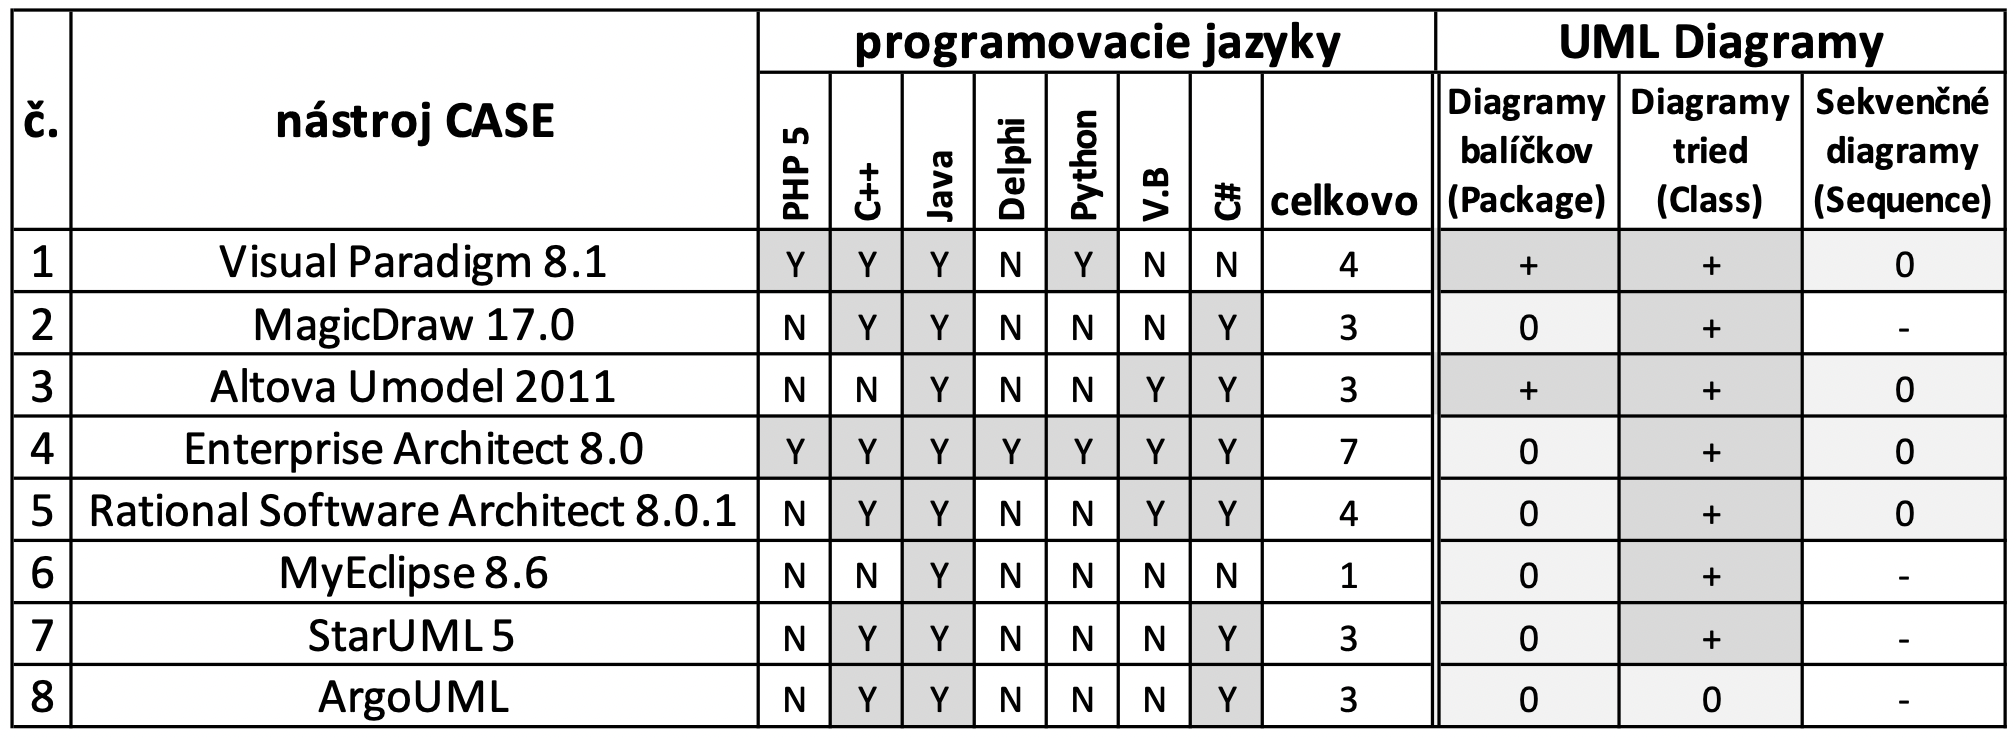
\includegraphics[width=1.2\textwidth]{tabulka_nastrojov.png}
\caption{Zoznam podporovaných programovacích jazykov a diagramov jednotlivými nástrojmi (prevzatá a upravená od \cite{Osman:RE})}
\label{tabulka2}
\end{table}
 
 Väčšina nástrojov je schopná spätnej rekonštrukcie diagramov balíčkov \emph{(package)}. Všetky porovnávané nástroje dokážu generovať diagramy tried \emph{(class)}, ArgoUML je však v tomto najmenej spoľahlivý, keďže nedokáže rekonštruovať vzťahy medzi triedami (iné ako dedičnosť) \cite{Osman:RE}. Čo sa týka sekvenčných diagramov, ani pri jednom z porovnávaných nástrojov sa nedá hovoriť o priamej podpore, no niektoré nástroje dokážu s malou pomocou používateľa generovať takéto diagramy.
 
 \section{Reakcia na témy z prednášok}
 %--- reakcia na tému ``Udržateľnosť a etika'' odtialto ---
\paragraph{Udržateľnosť a etika.} 
O udržateľnosti, z hľadiska softvéru, by sa dalo povedať ako o schopnosti pretrvať. To znamená, že softvér bude v budúcnosti dostupný (napr. nová platforma). Na to je samozrejme potrebné ho udržiavať. Práve nástroje, schopné reverzného inžinierstva dokážu veľmi pomôcť pri údržbe softvéru, kde pomáhajú s pochopením samotného systému. Vďaka nim je možné extrahovať štruktúru programu. 

Táto metóda môže byť využitá aj v kontexte etiky, pri detekcii plagiátorstva, kedy štruktúra programu môže slúžiť ako ukazovateľ príliš veľkej podobnosti (alebo zhodnosti). Pri skopírovaní cudzej práce a prezentovaní ju za svoju by bolo možné získať podobnú (prípadne rovnakú) štruktúru. Na identifikáciu plagiátorstva určite existuje veľa nástrojov, ktoré ponúkajú presnejšie výsledky, ale je zrejmé, že výsledky reverzného inžinierstva môžu slúžiť ako podnet k ďalšiemu prešetreniu.
%--- potialto je reakcia na tému z prednášky ``udržateľnosť a etika'' ---


 %--- reakcia na tému ``Technológia a ľudia'' odtialto ---
 \paragraph{Technológia a ľudia.}
Technológia ako pojem navodzuje pocit hmotného objektu. Významovo ale môže predstavovať aj softvérové riešenie. Je dôležité vedieť technológie využívať vo svoj prospech, a teda tak aby slúžili ľuďom a nie naopak. Technológie umožňujú ľuďom pracovať efektívnejšie prostredníctvom automatizácie, ktorú im ponúkajú. Rovnako tak aj nástroje CASE ponúkajú automatizáciu v rôznych fázach SDLC. Sú odpoveďou na stále narastajúce nároky a zvyšujúcu sa komplexnosť počítačových systémov. Náklady na vývoj softvéru každým rokom narastajú, a preto, ako aj autor~\cite{2001} uvádza, už len skromné vylepšenia pri vývoji a automatizácii môžu znamenať veľké úspory. Vďaka automatizácii, ktorú ponúkaju, dokážu pomôcť pri vývoji vysokokvalitného softvéru načas a v súlade s rozpočtom.
 %--- potialto je reakcia na tému z prednášky ``technológia a ľudia'' ---
 
 % ---reakcia na tému ``História informatiky'' odtialto-----
 \paragraph{Historické súvislosti.}
 V dnešnej dobe veľa vecí berieme ako samozrejmosť a neuvedomujeme si, koľko času a úsilia ľudia venovali týmto pre nás maličkostiam. Iné to nie je ani v informatike. Zoberme si napríklad pre nás úplne bežnú vec, že na jednom zariadení dokáže bežať niekoľko programov súčasne. V začiatkoch informatiky to nebolo také samozrejmé. Softvér na počítačoch bol minimálny a často si ho používateľ musel vytvroiť sám. Takto špecificky naprogramovaný počítač dokázal pracovať iba s jedným programom. V 50. rokoch minulého storočia boli počítače nanjvýš tak vo veľkých spoločnostiach, výskumných centrách a na univerzitách. Na jednej takej univerzite, konkrétne na MIT, videl Fernando Corbató potenciál drahého prístroja, ktorý zatiaľčo je zaneprázdnený nenáročnými výpočtami zostáva nevyužitý, a preto sa rozhodol vytvoriť akýsi operačný systém, ktorý by dovoľoval pracovať súbežne viacerým používateľom na jednom počítači. V roku 1961 predstavil takýto operačný systém pod názvom Compatible Time-Sharing System (CTSS). Z neho sa vyvinul operačný systém Multics, ktorý bol neskôr inšpiráciou pre vytvorenie operačného systému Unix. 
 %--- potialto ----
 
\section{Zhrnutie} \label{zhrnutie} 
Tento článok skúmal automatizáciu SDLC pomocu nástrojov CASE. Boli uvedené dve rôzne klasifikácie, na základe ktorých možno nástroje CASE rozdeliť. Obe síce vychádzajú z jednotlivých fáz životného cyklu, no jedno delí nástroje podľa konkrétnych fáz a druhé ich zase stručnejšie delí do ranných a neskorých fáz.
V práci je ďalej opísané tzv. \emph{dopredné} inžinierstvo a potreba zavedenia tohto prídavného mena. Neskôr je v článku popísané aj reverzné inžinierstvo a stručne uvedená potreba jeho využitia. 
V posledných častiach sa článok zameriava na ohodnotenie 8 konkrétnych nástrojov CASE (z  toho 6 komerčných a 2 open source) v reverznom inžinierstve. Pri porovnávaní bolo sledované, aké programovacie jazyky sú nástrojom podporované, a tiež ktoré typy diagramov sú podporované. Pri typoch diagramoch boli nástroje hodnotené aj na základe toho, ako úspešne dokázali jednotlivé typy diagramov rekonštruovať. Nasledujúce závery sú prevzaté od~\cite{Osman:RE}.

Z výsledkov porovnania vyplýva, že všetky nástroje dokážu rekonštruovať diagramy tried a diagramy balíčkov zo zdrojového kódu. Niektoré nástroje produkujú aj sekvenčné diagramy, no pri nich sa nejedná o úplne automatické generovanie (používateľ musí vybrať metódu v triede).

Celkovo neboli pozorované veľke rozdiely medzi schopnosťami jednotlivých nástrojov. Všetky majú relatívne rovnaké silné a slabé stránky. Jedna slabina bola pozorovaá naprieč všetkými porovnávanými nástrojmi. Ide o nesprávne zobrazenie vzťahov medzi triedami, kde agregáciu a kompozíciu často prezentujú ako asociáciu (prípadne neprezentujú vôbec). Takýto informačný chaos môže viesť k nesprávnej interpretácii. Používatelia, ktorí chcú využívať tieto nástroje v reverznom inžinierstve by si mali byť vedomí tohoto nedostatku.

Do budúcna sa odporúča zopakovať toto porovnanie, prípadne porovnať nástroje prezentované v tejto práci s inými nástrojmi, nakoľko výsledky štúdie, ktoré dosiahli Osman a Chaudron sa môžu zdať zastarané. Vďaka nim ale ich nasledovníci vedia, aké parametre treba detailne odsledovať.

V závere článku možno nájsť reakcie na témy z predmetu Metódy inžinierskej práce. Témy \emph{Udržateľnosť a etika} a \emph{Technológia a ľudia} nadväzujú na článok. Pri téme \emph{Historické súvislosti} je vyjadrenie ku konkrétnej osobnosti z prednášky.


%\acknowledgement{Ak niekomu chcete poďakovať\ldots}


% týmto sa generuje zoznam literatúry z obsahu súboru literatura.bib podľa toho, na čo sa v článku odkazujete
\bibliography{literatura}
\bibliographystyle{abbrv} % prípadne alpha, abbrv alebo hociktorý iný
\end{document}
